\documentclass[12pt]{article}
\usepackage{fontspec}
\usepackage{polyglossia}
\setdefaultlanguage{russian}
\setmainfont[Mapping=tex-text]{CMU Serif}

\begin{document}
%% Весь этот текст можно удалить
%% ====== от сих =====
\centering {\LARGE Формальные языки}

{\Large домашнее задание до 23:59 14.03}
\bigskip

\enumerate
{
  \item
  { Построить минимальные автоматы, распознающие пересечение, объединение и разность языков, распознаваемых следующими автоматами.
  

          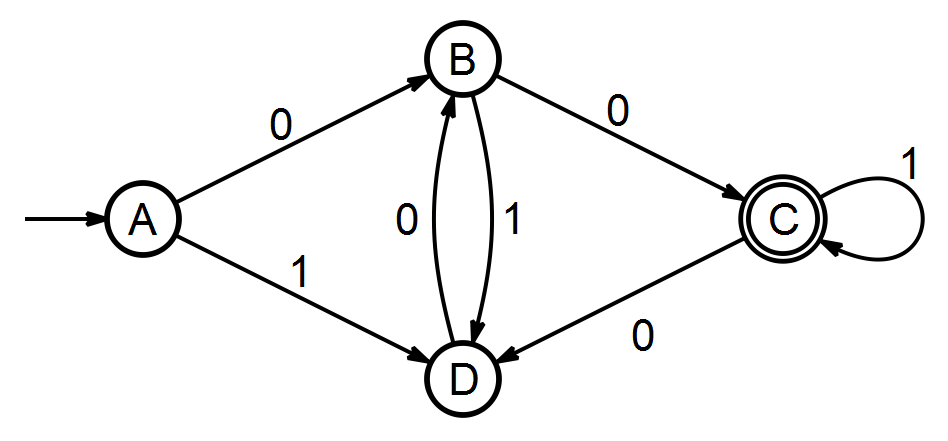
\includegraphics[width=250pt]{2_0.png}

~\\~

          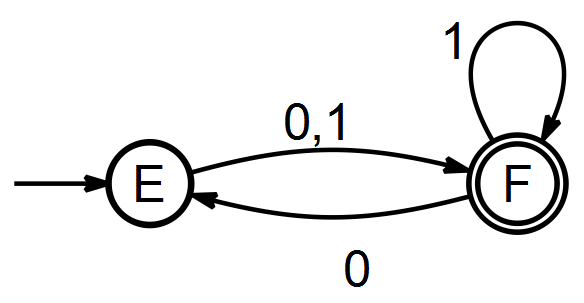
\includegraphics[width=150pt]{2_1.png} 

  }
    
  \item Детерминизировать следующие автоматы, построить их произведение. Минимизировать автоматы, если это необходимо. 
  
  \centering { 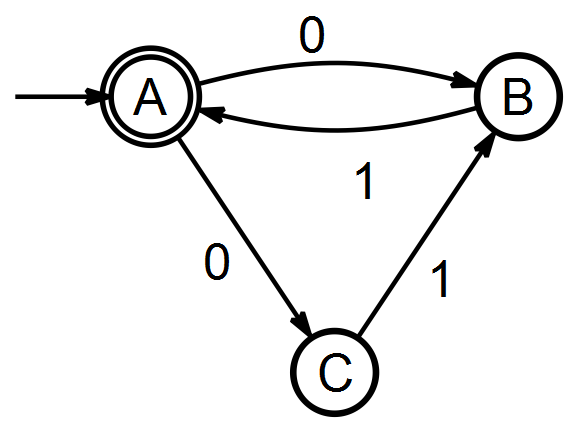
\includegraphics[width=150pt]{3.png}   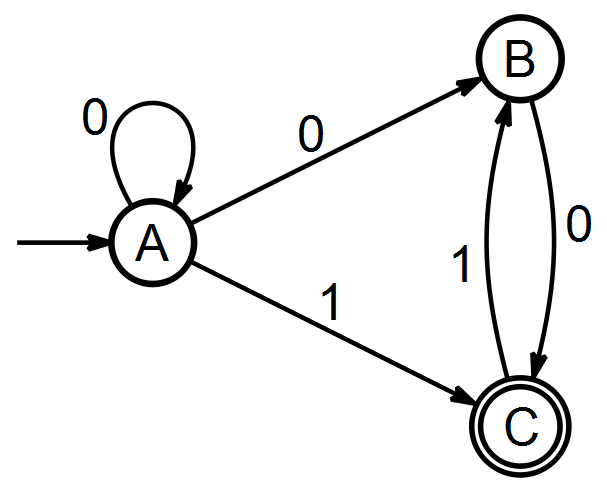
\includegraphics[width=150pt]{4.png} }
}

%% ===== и до сих =====
\end{document}
